\subsection{Magnetismo}

Tal vez el concepto de polos magnéticos parezca similar al de carga eléctrica, y los polos norte y sur parezcan análogos a las cargas positiva y negativa. No obstante, tal analogía puede ser errónea. Si bien las cargas positiva y negativa existen aisladas, no hay evidencia experimental de que exista un polo magnético aislado.

Los imanes siempre se encuentran como dipolos magnéticos (norte y sur), y no se ha comprobado la existencia los monopolos magnéticos.

\subsubsection{Campo Magnético}

Al igual que el campo eléctrico, el magnético es un \hl{\textit{campo vectorial}}, es decir, una cantidad vectorial asociada con cada punto del espacio. La existencia de un campo magnético en algún punto del espacio puede determinarse midiendo la magnitud de la \textbf{fuerza magnética} que ejerce el campo sobre una partícula de prueba ubicada en ese punto.

En esencia el magnetismo es un fenómeno físico asociado al movimiento de cargas eléctricas, que da lugar a fuerzas de atracción o repulsión entre materiales. Se manifiesta principalmente a través de los campos magnéticos, los cuales son representaciones vectoriales que describen la influencia que una corriente eléctrica o un material magnético ejerce en su entorno.

Desde un punto de vista fundamental, \hl{el origen del magnetismo reside en el movimiento de cargas eléctricas} a nivel microscópico, particularmente en el espín y el momento orbital de los electrones en los átomos. En materiales como el hierro, cobalto y níquel, estos momentos magnéticos atómicos se alinean de manera colectiva, generando imanes permanentes.

El \textbf{campo magnético} se representa mediante el vector \(\vec{B}\), cuya unidad en el Sistema Internacional es el tesla (T)\footnote{Un tesla equivale a: \(T \equiv \frac{Ns}{Cm} \equiv \frac{N}{Am}\)}. La interacción de una carga en \textbf{movimiento} \(q\) con un campo magnético está regida por la fuerza magnética, expresada como:
\begin{equation}
  \vec{F}_B = q\vec{v} \times \vec{B}
  \label{eq:fuerza_magnética}
\end{equation}
donde \(\vec{v}\) es el vector velocidad de la partícula. Esta fuerza es perpendicular tanto a la dirección de la velocidad como a la del campo magnético.

\begin{figure}[ht]
  \centering
  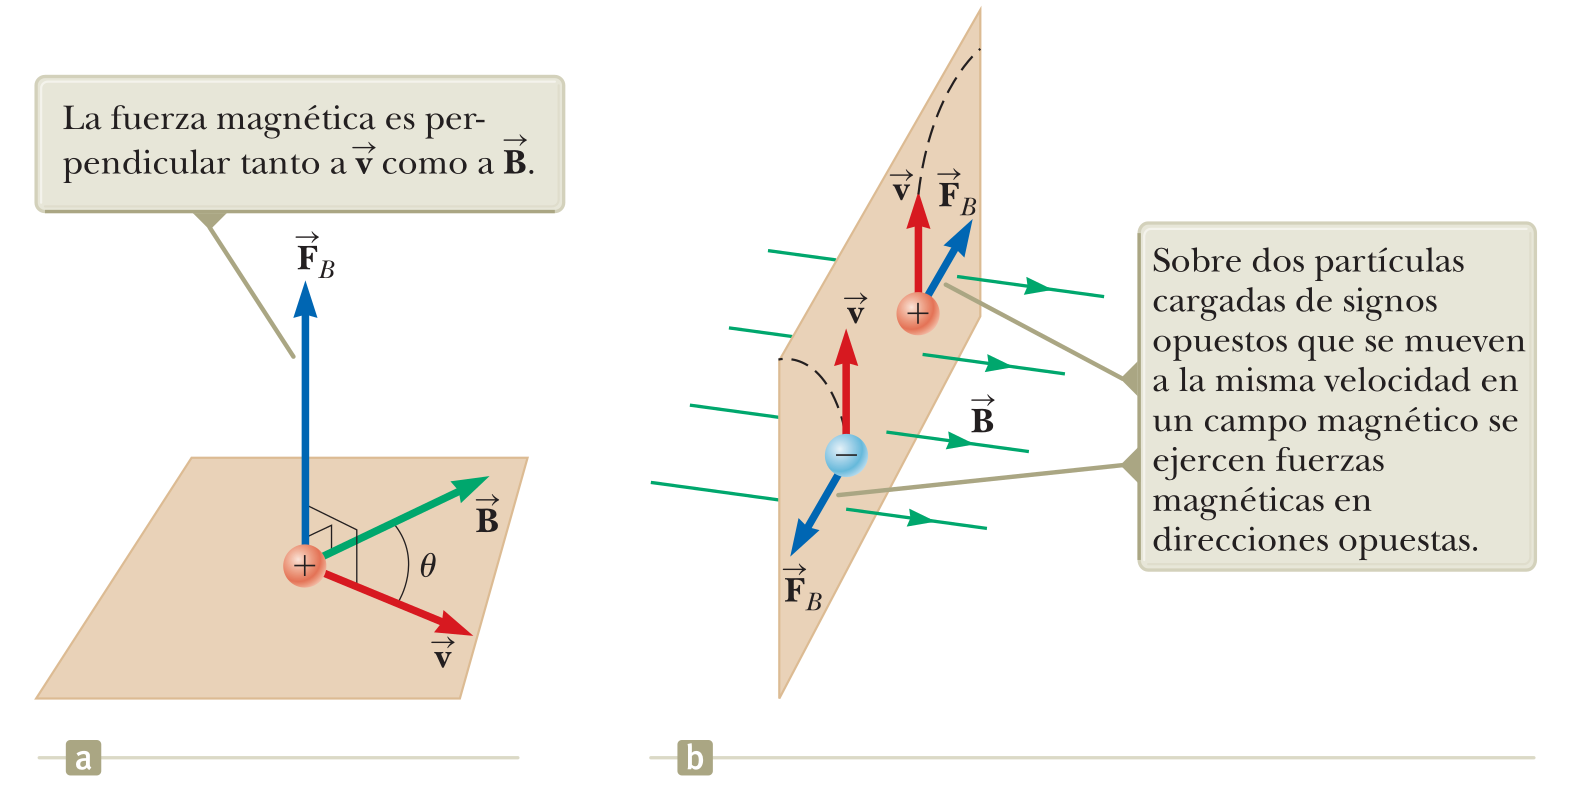
\includegraphics[width=0.8\textwidth]{magnetic_force.png}
  \caption{Partículas con carga atravesando un campo magnético \(\vec{B}\) con una velocidad \(\vec{v}\)}
\end{figure}

Si se conoce el ángulo \(\theta\) entre el vector velocidad \(\vec{v}\) y el campo magnético \(\vec{B}\) la fuerza se puede calcular como:
\[
  \vec{F}_B = \left\lvert q \right\rvert v B \sin(\theta) \hat{r}
\]
donde \(\hat{r}\) es un versor\footnote{versor: vector de módulo 1} normal al plano formado por los vectores \(\vec{v}\) y \(\vec{B}\). 

Comparando la fuerza magnética con la fuerza eléctrica se puede ver que la fuerza \(\vec{F}_B\) es perpendicular al campo magnético y a la velocidad de la partícula, mientras que \(\vec{F}_e\) se ejerce sobre la dirección del campo eléctrico. Además \(\vec{F}_e\) no requiere que la partícula con carga esté en movimiento.

\subsubsection{Lineas de campo magnético}

\begin{wrapfigure}{r}{0.3\textwidth}
  \centering
  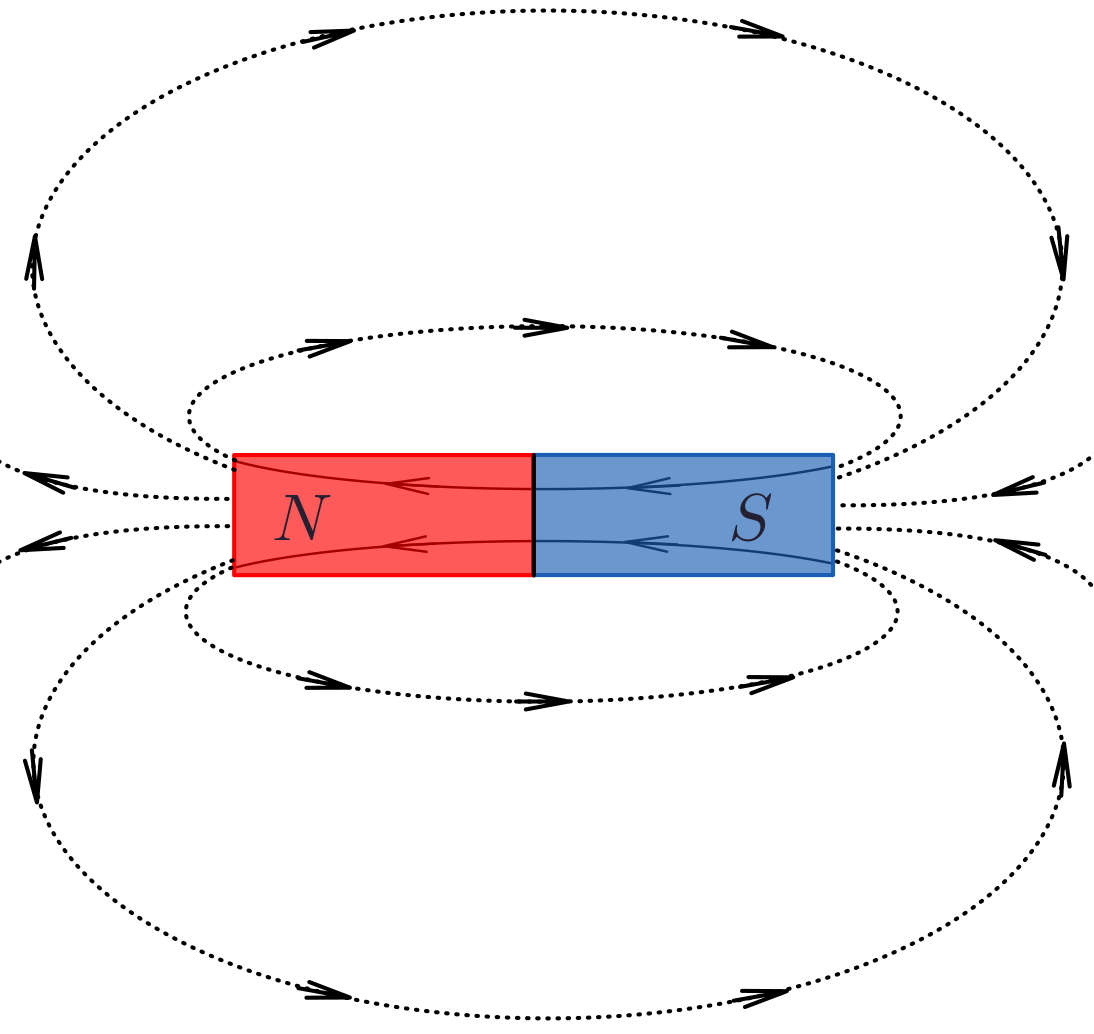
\includegraphics[width=\linewidth]{magnetic_field_lines.png}
  \caption{Líneas de campo magnético.}
  \label{fig:lineas_de_iman}
\end{wrapfigure}
La representación de los campos magnéticos mediante líneas de campo magnético es muy útil para visualizar la intensidad y la dirección del campo magnético. Como se muestra en la figura \ref{fig:lineas_de_iman}, cada una de estas líneas forma un bucle cerrado, aunque no se muestren todas las líneas cerradas por las limitaciones del espacio disponible puede observarse en las líneas de campo más cercanas al cuerpo del imán que salen del polo norte (\(N\)), hacen un bucle hacia el polo sur (\(S\)) y continúan a través de la barra magnética de vuelta al polo norte. Dentro del imán las líneas están muy juntas, pero nunca se cortan o tocan entre sí.

Las líneas de campo magnético tienen varias reglas estrictas:
\begin{enumerate}
  \item La dirección del campo magnético \(\vec{B}\) es tangente a la línea de campo en cualquier punto del espacio. Una pequeña brújula señalará la dirección de la línea del campo.
  \item La fuerza del campo es proporcional a la cercanía de las líneas. Es exactamente proporcional al número de líneas por unidad de superficie perpendicular a las líneas (llamada densidad de área). Es el mismo concepto que en las líneas de campo eléctrico. Mientras más juntas están mayor intensidad tiene.
  \item Las líneas de campo magnético no pueden cruzarse nunca, lo que significa que el campo es único en cualquier punto del espacio.
  \item Las líneas de campo magnético son continuas, formando bucles cerrados sin principio ni fin. Se dirigen del polo norte al polo sur.
\end{enumerate}

La última propiedad está relacionada con el hecho de que los polos norte y sur no pueden separarse. Es una diferencia clara respecto a las líneas de campo eléctrico, que generalmente comienzan en cargas positivas y terminan en cargas negativas o en el infinito. Si existieran cargas magnéticas aisladas (denominadas monopolos magnéticos), las líneas de campo magnético comenzarían y terminarían en ellas. Puedes ver más ejemplos sobre líneas de campo magnético en \href{https://openstax.org/books/f%C3%ADsica-universitaria-volumen-2/pages/11-2-campos-y-lineas-magneticas}{OpenStax} (\cite{openstax})

\begin{figure}[ht]
  \centering
  \begin{subfigure}[b]{0.35\textwidth}
      \centering
      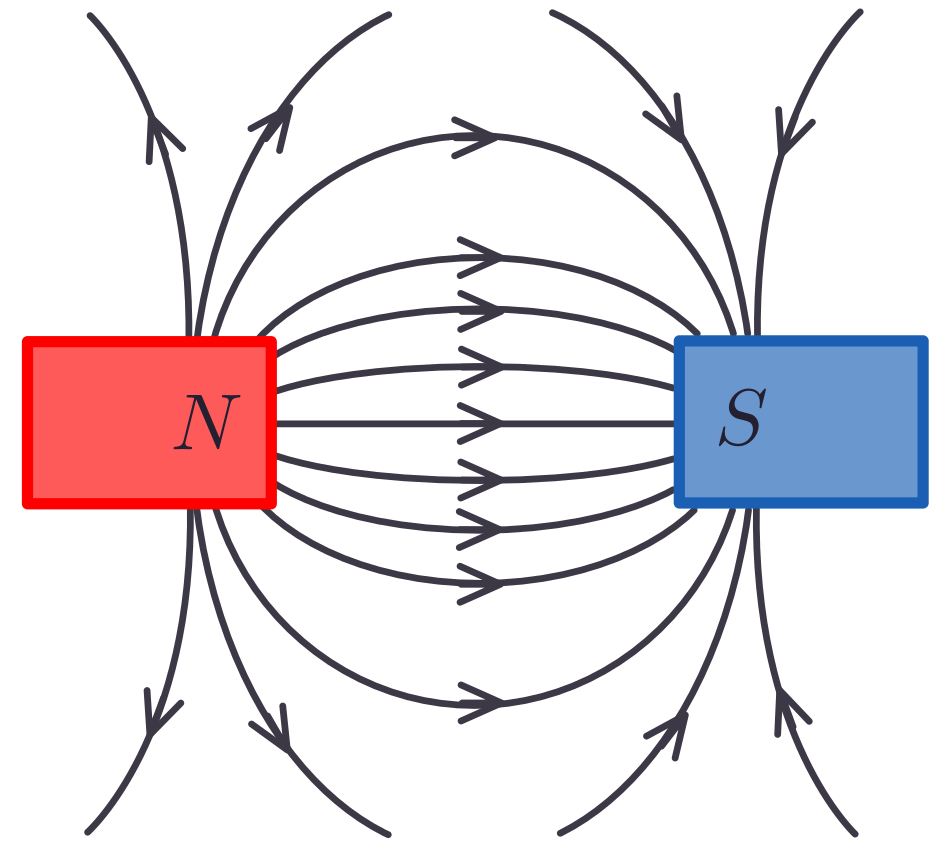
\includegraphics[width=\textwidth]{magnetic_lines_a.png}
      \caption{Líneas de campo magnético entre polos opuestos.}
      \label{fig:polos_opuestos}
  \end{subfigure}
  \hspace{10pt}
  \begin{subfigure}[b]{0.35\textwidth}
      \centering
      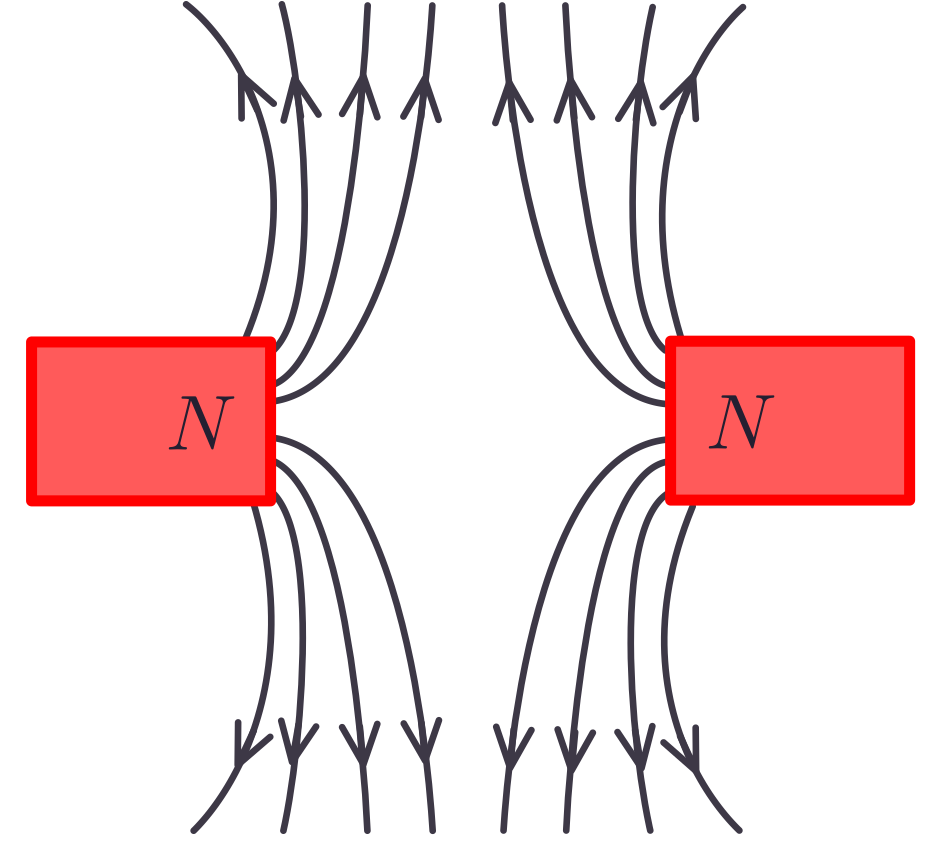
\includegraphics[width=\textwidth]{magnetic_lines_b.png}
      \caption{Líneas de campo magnético entre polos similares.}
      \label{fig:polos_iguales}
  \end{subfigure}
  \caption{Lineas de campo para distintas configuraciones de imanes.}
  \label{fig:lineas_de_campo_magnético_entre_imanes}
\end{figure}

Como se puede observar en la figura \ref{fig:lineas_de_campo_magnético_entre_imanes} las líneas de campo magnético se definen para tener la dirección en la que apunta una pequeña brújula cuando se coloca en un lugar del campo. La fuerza del campo es proporcional a la cercanía (o densidad) de las líneas. Si se pudiera sondear el interior del imán, se encontraría que las líneas de campo forman bucles continuos y cerrados. Para ajustarse a un espacio razonable, algunos de estos dibujos pueden no mostrar el cierre de los bucles; sin embargo, si se dispusiera de espacio suficiente, los bucles estarían cerrados. 

Nótese que en la figura \ref{fig:polos_opuestos} el campo que se forma en el centro de los imanes es casi uniforme. Este concepto es útil ya que este tipo de campo se encuentra en los imanes de herradura (como el que está en la figura \ref{fig:iman}). Por otro lado en la figura \ref{fig:polos_iguales} el campo entre imanes es casi cero (muy poca intensidad) ya que las líneas de campo magnético están muy separadas entre sí.

\subsubsection{Flujo Magnético}
\label{sec:flujo_magnético}

Definimos el \textbf{flujo magnético} \(\Phi_B\) a través de una superficie igual que definimos el flujo eléctrico en relación con la ley de Gauss en la sección \ref{sec:flujo_electrico}. 

El flujo magnético es una magnitud escalar que cuantifica la cantidad de campo magnético que atraviesa una superficie dada. Matemáticamente, se define como la integral del producto escalar entre el campo magnético \(\vec{B}\) y el vector diferencial de área \(d\vec{A}\) de la superficie:

\[
\Phi_B = \int_S \vec{B} \cdot d\vec{A}
\]
donde:
\begin{itemize}
  \item \(\Phi_B\) es el flujo magnético,
  \item \(S\) es la superficie sobre la que se calcula el flujo,
  \item \(\vec{B}\) es el vector del campo magnético,
  \item \(d\vec{A}\) es un elemento diferencial de área, cuyo módulo es el área diferencial y cuya dirección es perpendicular a la superficie, siguiendo la convención del sentido positivo (normal saliente en una superficie cerrada).
\end{itemize}

Al igual que el flujo eléctrico, el flujo magnético mide cuántas ``líneas de campo magnético'' atraviesan una superficie. Si el campo es perpendicular a la superficie, el flujo es máximo; si es paralelo, el flujo es nulo.

En el caso especial donde el campo magnético es uniforme y la superficie es plana, la expresión se simplifica a:
\[
\Phi_B = B A \cos\theta
\]
donde:
\begin{itemize}
  \item \(B\) es la magnitud del campo magnético,
  \item \(A\) es el área de la superficie,
  \item \(\theta\) es el ángulo entre el vector \(\vec{B}\) y el vector normal a la superficie.
\end{itemize}

La unidad de flujo magnético en el Sistema Internacional es el weber (Wb), donde: \(1 \, \text{Wb} = 1 \, \text{T} \cdot \text{m}^2\)

Si recuerda el \textit{flujo eléctrico} y la ley de Gauss de la sección \ref{sec:ley_de_gauss} podríamos intuir que para el magnetismo pasa algo similar. Sin embargo como no existen los monopolos magnéticos y las líneas de campo magnético son cerradas \hl{el flujo magnético sobre una superficie cerrada es siempre cero.}
\[
\oint \vec{B}\cdot d\vec{A} = 0
\]
Digamos, en palabras simples: si encerramos un imán en una superficie Gaussiana, todas las líneas de campo magnético que salen, vuelven a entrar. Esto resulta en un flujo nulo.

\subsubsection{Trabajo del campo magnético}

En la sección \ref{sec:potencial} vimos como una carga que se mueve en un campo eléctrico realiza un trabajo. En esta sección las partículas deben estar si o si en movimiento para verse afectadas por el campo magnético. Entonces ¿Será que están realizando trabajo? La respuesta rápida es que no. Veamos el por qué: recordando que el trabajo es el \textbf{producto escalar} entre la fuerza por la distancia (o desplazamiento), si la fuerza es perpendicular al desplazamiento entonces dará siempre cero.
En base a esto, vemos que \(\vec{F}_B\) no realiza trabajo ni cambia la energía del sistema carga-campo por ser perpendicular al plano de \(\vec{B}\) y \(\vec{v}\). 

\begin{tcolorbox}[myconclusion]
  Con base en este último enunciado y también con el teorema trabajo-energía cinética, se concluye que la energía cinética de una partícula cargada que se mueve a través de un campo magnético \textbf{no} puede ser modificada sólo por el campo magnético. El campo magnético puede modificar la dirección del vector velocidad, pero no puede cambiar la rapidez ni la energía cinética de la partícula.
\end{tcolorbox}

\begin{wrapfigure}{l}{0.3\textwidth}
  \centering
  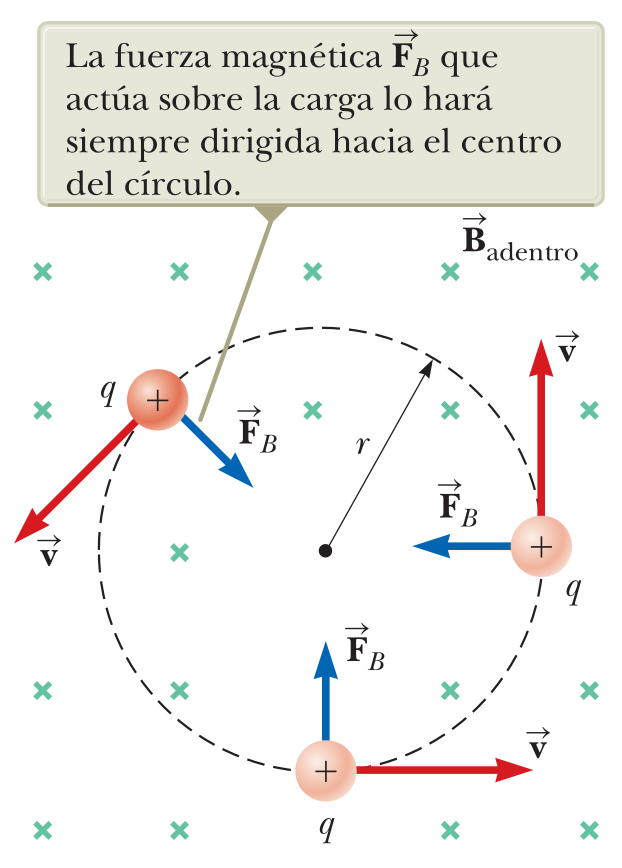
\includegraphics[width=\linewidth]{centipet_force.png}
  \caption{Fuerza magnética para una partícula con velocidad \(v\) y un campo magnético entrante.}
  \label{fig:centripet_force}
\end{wrapfigure}
\subparagraph{Pregunta:}

\noindent ¿Qué tipo de fuerza es siempre perpendicular a la trayectoria de una partícula y no modifica la magnitud de la velocidad?

\vspace{3pt}

\noindent La \textbf{fuerza centrípeta}. Entonces, la fuerza magnética, como se ve en la figura \ref{fig:centripet_force} es una fuerza centrípeta para una partícula cargada y en movimiento. Por lo tanto podemos ocupar todas las ecuaciones del movimiento circular.

Si no recuerdas bien los temas de dinámica y las ecuaciones del movimiento circular uniforme y no uniforme puedes volver a verlo en la sección \ref{sec:mcu}

Con este principio, se observa que para la situación ilustrada en la figura \ref{fig:centripet_force} la magnitud de \(\vec{F}_B\) y \(\vec{v}\) son constantes. Como \(\vec{F}_B \equiv \vec{F}_c\) entonces podemos igualar \(\vec{F}_B\) a la expresión de aceleración centrípeta:
\[
  F_B = qvB = m \frac{v^2}{r}
\]